
%%%%%%%%%%%%%%%%%%%%%%% file typeinst.tex %%%%%%%%%%%%%%%%%%%%%%%%%
%
% This is the LaTeX source for the instructions to authors using
% the LaTeX document class 'llncs.cls' for contributions to
% the Lecture Notes in Computer Sciences series.
% http://www.springer.com/lncs       Springer Heidelberg 2006/05/04
%
% It may be used as a template for your own input - copy it
% to a new file with a new name and use it as the basis
% for your article.
%
% NB: the document class 'llncs' has its own and detailed documentation, see
% ftp://ftp.springer.de/data/pubftp/pub/tex/latex/llncs/latex2e/llncsdoc.pdf
%
%%%%%%%%%%%%%%%%%%%%%%%%%%%%%%%%%%%%%%%%%%%%%%%%%%%%%%%%%%%%%%%%%%%


\documentclass[11pt]{article}\usepackage[]{graphicx}\usepackage[]{color}
%% maxwidth is the original width if it is less than linewidth
%% otherwise use linewidth (to make sure the graphics do not exceed the margin)
\makeatletter
\def\maxwidth{ %
  \ifdim\Gin@nat@width>\linewidth
    \linewidth
  \else
    \Gin@nat@width
  \fi
}
\makeatother

\definecolor{fgcolor}{rgb}{0.345, 0.345, 0.345}
\newcommand{\hlnum}[1]{\textcolor[rgb]{0.686,0.059,0.569}{#1}}%
\newcommand{\hlstr}[1]{\textcolor[rgb]{0.192,0.494,0.8}{#1}}%
\newcommand{\hlcom}[1]{\textcolor[rgb]{0.678,0.584,0.686}{\textit{#1}}}%
\newcommand{\hlopt}[1]{\textcolor[rgb]{0,0,0}{#1}}%
\newcommand{\hlstd}[1]{\textcolor[rgb]{0.345,0.345,0.345}{#1}}%
\newcommand{\hlkwa}[1]{\textcolor[rgb]{0.161,0.373,0.58}{\textbf{#1}}}%
\newcommand{\hlkwb}[1]{\textcolor[rgb]{0.69,0.353,0.396}{#1}}%
\newcommand{\hlkwc}[1]{\textcolor[rgb]{0.333,0.667,0.333}{#1}}%
\newcommand{\hlkwd}[1]{\textcolor[rgb]{0.737,0.353,0.396}{\textbf{#1}}}%
\let\hlipl\hlkwb

\usepackage{framed}
\makeatletter
\newenvironment{kframe}{%
 \def\at@end@of@kframe{}%
 \ifinner\ifhmode%
  \def\at@end@of@kframe{\end{minipage}}%
  \begin{minipage}{\columnwidth}%
 \fi\fi%
 \def\FrameCommand##1{\hskip\@totalleftmargin \hskip-\fboxsep
 \colorbox{shadecolor}{##1}\hskip-\fboxsep
     % There is no \\@totalrightmargin, so:
     \hskip-\linewidth \hskip-\@totalleftmargin \hskip\columnwidth}%
 \MakeFramed {\advance\hsize-\width
   \@totalleftmargin\z@ \linewidth\hsize
   \@setminipage}}%
 {\par\unskip\endMakeFramed%
 \at@end@of@kframe}
\makeatother

\definecolor{shadecolor}{rgb}{.97, .97, .97}
\definecolor{messagecolor}{rgb}{0, 0, 0}
\definecolor{warningcolor}{rgb}{1, 0, 1}
\definecolor{errorcolor}{rgb}{1, 0, 0}
\newenvironment{knitrout}{}{} % an empty environment to be redefined in TeX

\usepackage{alltt}
%\newcommand{\bth}{\bm{\theta}}
\newcommand{\la}{\lambda}
\newcommand{\bl}{\bm{\lambda}}
%\newcommand{\bxi}{\bm{\xi}}
\newcommand{\bsee}{\bm{\Sigma_e}}
\newcommand{\bo}{\bm{\Omega}}
\newcommand{\bD}{\bm{\Delta}}
%\newcommand{\bse}{\bm{\Sigma_e}^{-1}}
\newcommand{\bT}{\bm{t}}
%\newcommand{\bh}{\bm{H}}
\newcommand{\bc}{\bm{C}}
%\newcommand{\bd}{\bm{D}}
\newcommand{\bww}{\bm{W}}
%\newcommand{\ba}{\bm{A}}
\newcommand{\bbb}{\bm{B}}
\newcommand{\bg}{\bm{G}}
\newcommand{\bmy}{\bm{y}}
%\newcommand{\bys}{\bm{y^*}}
\newcommand{\bdd}{\bm{\delta}}
\newcommand{\bdh}{\hat{\bm{\delta}}}
%\newcommand{\byst}{\bm{y^{*T}}}

\newcommand{\thatb}{\hat{\bm{\theta}}^B}
\newcommand{\thatt}{\hat{\bm{\theta}}}
\newcommand{\thattt}{\hat{\bm{\theta_2}}}
\newcommand{\thp}{\hat{\bm{\theta}}^p}
\newcommand{\thg}{\hat{\bm{\theta}}^g}
\newcommand{\thbm}{\hat{\bm{\theta}}^{BM}}

\newcommand{\bty}{\tilde{\bm{\theta}}_{y,t}}
\newcommand{\su}{{\sigma_u^2}}
\newcommand{\thh}{{\theta}}
\newcommand{\bgam}{\bm{\gamma}}
\newcommand{\bth}{\bm{\theta}}
\newcommand{\bxi}{\bm{x}_i}
\newcommand{\bse}{\bm{\Sigma_e}^{-1}}
\newcommand{\bh}{\bm{H}}
\newcommand{\bd}{\bm{D}}
%\newcommand{\ba}{\bm{A}}
\newcommand{\bb}{\bm{\beta}}
% y\newcommand{\bxi}{\bm{x}_i}
\newcommand{\bys}{\bm{y^*}}
\newcommand{\byst}{\bm{y^{*T}}}
\newcommand{\V}       {\text{Var}}
\newcommand{\de}       {\mbox{$\delta_i$}}
\newcommand{\tij}       {\mbox{$\theta_{ij}$}}
\newcommand{\htijb}       {\mbox{$\hat{\theta}_{ij}^B$}}

\newcommand{\thbariw}     {\mbox{$\bar{\hat{\theta}}_{iw}^{B}$}}
\newcommand{\tbw}       {\mbox{$\bar{\theta}_{w}^B$}}
\newcommand{\tbiw}       {\mbox{$\bar{\theta}_{iw}$}}
\newcommand{\thwb}       {\mbox{$\bar{\hat\bm{{\theta}}}_{w}^B$}}
\newcommand{\thw}       {\mbox{$\bar{\hat{\theta}}_{w}^B$}}
\newcommand{\thbiw}       {\mbox{$\bar{\hat{\theta}}_{iw}^B$}}
\newcommand{\that}       {\mbox{$\hat{\theta}$}}
\newcommand{\thij}       {\mbox{$\hat{\theta}_{ij}$}}
\newcommand{\thhi}       {\mbox{$\hat{\theta}_{i}$}}
\newcommand{\thi}       {\theta_i}

%\newcommand{\lt}       {\left}
%\newcommand{\rt}       {\right}
\newcommand{\lao}       {\mbox{$\lambda_{1i}$}}
\newcommand{\lat}       {\mbox{$\lambda_{2}$}}
\newcommand{\latt}       {\mbox{$\lambda_{3i}$}}


\newcommand{\cd}{\buildrel d \over \longrightarrow}
\newcommand{\cp}{\buildrel P \over \longrightarrow}
%\newcommand{\R}{\mathbb{R}}
\newcommand{\hatbb}{\boldsymbol{\hat{b}}}
\newcommand{\hatbB}{\boldsymbol{\hat{B}}}
\newcommand{\hatbd}{\boldsymbol{\hat{d}}}
\newcommand{\commentt}[1]{}
\newcommand{\myvfil}[1]{\vskip 0pt plus #1fill}
% \renewcommand{\upsilon}{v}
\newcommand{\lik}{\ell_y(\theta)}
\newcommand{\likil}{\ell_y(\theta_i^{(l)})}
\newcommand{\hd}{\hfill$\diamondsuit$}
\newcommand{\aaa}{\epsilon}
\newcommand{\lt}{\left}
\newcommand{\rt}{\right}
\newcommand{\mbi}{\max_{1 \leq i \leq m} \bxi'\bb}
\newcommand{\bs}{B_{i*}}
\newcommand{\D}{\Delta}
\newcommand{\bi}{B_{i}}
%\newcommand{\that}        {\mbox{$\hat{\boldsymbol{\theta}}$}}
\newcommand{\utheta}        {\mbox{$\boldsymbol{\theta}$}}
\newcommand{\thhj}{\hat{\theta}_j}
\newcommand{\thhij}{\hat{\theta}_{ij}}
\newcommand{\thiHB}{\hat{\theta}_i^{HB}}
\newcommand{\thih}{\hat{\theta}_i^H}
\newcommand{\thit}{\tilde{\theta}_i^H}
%\newcommand{\V}{\text{Var}}

\newcommand{\tr}{\text{tr}}
\newcommand{\btt}{\boldsymbol{\theta}}

\newcommand{\ttt}{\boldsymbol{t}}
\newcommand{\bhat}{\boldsymbol{\hat{\beta}}}
\newcommand{\thb}{\bar{\theta}}
\newcommand{\bx}{\bm{x}}
\newcommand{\bX}{\bm{X}}
\newcommand{\bY}{\boldsymbol{Y}}
\newcommand{\lam}{\boldsymbol{\Lambda}}
\newcommand{\pxv}{{P}_X^V}
\newcommand{\pxvt}{\bar{P}_x^{V'}}
\newcommand{\pxvs}{\bar{P}_x^{V_*}}
\newcommand{\bv}{\boldsymbol{v}}
\newcommand{\bu}{\boldsymbol{u}}
\newcommand{\ur}{\boldsymbol{r}}
\newcommand{\uphi}{\boldsymbol{\phi}}
\newcommand{\uone}{\boldsymbol{1}}
\newcommand{\ue}{\boldsymbol{e}}
\newcommand{\uc}{\boldsymbol{c}}
\newcommand{\bbi}{\boldsymbol{b}_i}
\newcommand{\uw}{\boldsymbol{w}}
\newcommand{\bz}{\boldsymbol{z}}
\newcommand{\be}{\boldsymbol{e}}
\newcommand{\by}{\boldsymbol{y}}
\newcommand{\utt}{\boldsymbol{t}}
\newcommand{\bzero}{\boldsymbol{0}}
%\newcommand{\bl}{\boldsymbol{l}}
\newcommand{\util}{\boldsymbol{\tilde{u}}}
\newcommand{\utils}{\boldsymbol{\tilde{u}_*}}
\newcommand{\btil}{\boldsymbol{\tilde{\beta}}}
\newcommand{\btils}{\boldsymbol{\tilde{\beta}^{*}}}
%\newcommand{\bm}{\boldsymbol{m}}
\newcommand{\btilf}{(X'V^{-1}X)^{-1}X'V^{-1}\that}
\newcommand{\btilfs}{(X'V_*^{-1}X)^{-1}X'V_*^{-1}\that}
\newcommand{\bxij}{\boldsymbol{x_{ij}}}
\newcommand{\bxj}{\boldsymbol{x_{j}}}
\newcommand{\bei}{\boldsymbol{e_{i}}}
\newcommand{\bej}{\boldsymbol{e_{j}}}
\newcommand{\bek}{\boldsymbol{e_{k}}}
\newcommand{\bbary}{\boldsymbol{\bar{y}}}
\newcommand{\thet}{\boldsymbol{\theta}}



%\newcommand{\lao}       {\mbox{$\lambda_{1i}$}}
%\newcommand{\lat}       {\mbox{$\lambda_{2}$}}
%\newcommand{\latt}       {\mbox{$\lambda_{3i}$}}


\newcommand{\vv}        {V^{-1}}
\newcommand{\vs}        {V^{-1}_*}
\newcommand{\vvs}        {V_{*}}
\newcommand{\sig}        {\Sigma}
\newcommand{\sm}        {\sqrt{m}}
%\newcommand{\thi}        {\theta_i}
%\newcommand{\thhi}        {\mbox{$\hat{\theta}_i$}}
\newcommand{\thhk}        {\mbox{$\hat{\theta}_k$}}
\newcommand{\thho}        {\mbox{$\hat{\theta}_1$}}
\newcommand{\thhm}        {\mbox{$\hat{\theta}_m$}}
\newcommand{\thj}        {\mbox{$\hat{\theta}_j$}}
%\newcommand{\thij}        {\mbox{$\hat{\theta}_{ij}$}}
\newcommand{\ttil}        {\mbox{$\tilde{\boldsymbol{\theta}}$}}

\newcommand{\thk}        {\mbox{$\hat{\theta}_k$}}
%\newcommand{\tij}       {\mbox{$\theta_{ij}$}}
\newcommand{\thbi}        {\mbox{$\hat{\theta}_i^B$}}
\newcommand{\thbis}        {\mbox{$\hat{\theta}_{i*}^B$}}
\newcommand{\thebis}        {\mbox{$\hat{\theta}_{i*}^{EB}$}}
\newcommand{\thebjs}        {\mbox{$\hat{\theta}_{j*}^{EB}$}}
\newcommand{\thbj}        {\mbox{$\hat{\theta}_j^B$}}
\newcommand{\thbjs}        {\mbox{$\hat{\theta}_{j*}^B$}}
\newcommand{\thbk}        {\mbox{$\hat{\theta}_k^B$}}
%\newcommand{\htijb}        {\mbox{$\hat{\theta}_{ij}^B$}}
\newcommand{\thebi}       {\mbox{$\hat{\theta}_i^{EB}$}}
\newcommand{\thebj}       {\mbox{$\hat{\theta}_j^{EB}$}}
\newcommand{\theblupi}    {\mbox{$\hat{\theta}_i^{EBM1}$}}
\newcommand{\thbmi}    {\mbox{$\hat{\theta}_i^{BM1}$}}
\newcommand{\theblupis}       {\mbox{$\hat{\theta}_{i*}^{EBM1}$}}

%\newcommand{\thbiw}       {\mbox{$\bar{\hat{\theta}}_{iw}^B$}}
\newcommand{\thhw}       {\mbox{$\bar{\hat{\theta}}_{w}$}}
%\newcommand{\thw}       {\mbox{$\bar{\hat{\theta}}_{w}^B$}}
%\newcommand{\tbiw}       {\mbox{$\bar{\theta}_{iw}$}}
%\newcommand{\thbariw}     {\mbox{$\bar{\hat{\theta}}_{iw}^{B}$}}
\newcommand{\thbarw}     {\mbox{$\bar{\hat{\theta}}_{w}^{B}$}}
\newcommand{\thbarwb}     {\mbox{$\bar{\hat{\theta}}_w^{B}$}}
\newcommand{\thbarwbs}     {\mbox{$\bar{\hat{\theta}}_{w*}^{B}$}}
\newcommand{\thbarweb}     {\mbox{$\bar{\hat{\theta}}_w^{EB}$}}
\newcommand{\thbarwebs}     {\mbox{$\bar{\hat{\theta}}_{w*}^{EB}$}}
%\newcommand{\se}     {\mbox{$\sigma_{ei}^2$}}
%\newcommand{\su}    {\sigma_u^2}
\newcommand{\sbb}     {\mbox{$\sigma_b^2$}}
\newcommand{\sut}     {\mbox{$\tilde{\sigma}_u^2$}}
\newcommand{\suh}     {\mbox{$\hat{\sigma}_u^2$}}
\newcommand{\sus}     {\mbox{${\sigma}_u^{*2}$}}
\newcommand{\sust}     {\mbox{$\tilde{\sigma}_u^{*2}$}}
%\newcommand{\btil}     {\mbox{$(X'V^{-1}X)^{-1}X'V^{-1}\boldface{\theta}$}}
\newcommand{\hvis}     {\mbox{$\boldsymbol{x}_i'(X'V^{-1}_*X)^{-1}\boldsymbol{x}_i$}}
\newcommand{\hvi}     {\mbox{$\boldsymbol{x}_i'(X'V^{-1}X)^{-1}\boldsymbol{x}_i$}}
\newcommand{\hij}     {\mbox{$\boldsymbol{x}_i'(X'X)^{-1}\boldsymbol{x}_j$}}
\newcommand{\hvk}     {\mbox{$\boldsymbol{x}_k'(X'V^{-1}X)^{-1}\boldsymbol{x}_k$}}
\newcommand{\hj}     {\max_{1\leq j \leq m} h_j}
\newcommand{\hi}     {\max_{1\leq i \leq m} h_i}
\newcommand{\hk}     {\mbox{$\boldsymbol{x}_k'(X'X)^{-1}\boldsymbol{x}_k$}}
\newcommand{\hvik}     {\mbox{$\boldsymbol{x}_i'(X'V^{-1}X)^{-1}\boldsymbol{x}_k$}}
\newcommand{\hii}     {\mbox{$\boldsymbol{x}_i'(X'X)^{-1}\boldsymbol{x}_i$}}
%\newcommand{\bt}     {\mbox{$\tilde{\bm{\beta}}$}}
\newcommand{\ut}     {\mbox{$\tilde{\boldsymbol{u}}$}}
\newcommand{\uts}     {\mbox{$\tilde{\boldsymbol{u}}_*$}}
\newcommand{\ub}     {\mbox{${\boldsymbol{u}}$}}
%\newcommand{\bb}     {\mbox{${\boldsymbol{\beta}}$}}
\newcommand{\li}     {\mbox{${\lambda_i}$}}
\newcommand{\lj}     {\mbox{${\lambda_j}$}}
\newcommand{\lk}     {\mbox{${\lambda_k}$}} 
\newcommand{\co}     {\text{Cov}}
\newcommand{\lp}     {\left(}
\newcommand{\rp}     {\right)}
\newcommand{\lb}     {\left[}
\newcommand{\rb}     {\right]}
\newcommand{\gos}     {G_1^{*}}
\newcommand{\gtos}     {G_2^{*}}
\newcommand{\gts}     {G_3^{*}}
%\newcommand{\g}     {\mbox{$X(X'V^{-1}X)^{-1}X'$}}
\newcommand{\xg}     {\mbox{$(X'V^{-1}X)^{-1}X'$}}
%\newcommand{\bxi}{\boldsymbol{x}_i}
\newcommand{\bw}{\boldsymbol{w}}
\newcommand{\bci}{\boldsymbol{c}_i}
\newcommand{\bgi}{\boldsymbol{g}_i}
\newcommand{\bxk}{\boldsymbol{x}_k}
\newcommand{\byi}{\boldsymbol{y}_i}
\newcommand{\bzi}{\boldsymbol{z}_i}
\newcommand{\bt}{\boldsymbol{\tilde{\beta}}}
\newcommand{\lai}     {\lambda_i}
\newcommand{\gai}     {\gamma_i}
\newcommand{\ma}     {\max_{1 \leq i \leq m}}
\newcommand{\mak}     {\max_{1 \leq k \leq m}}

\newcommand{\cov}     {\text{Cov}}

%%leila/aa commands


\newcommand{\zv}{{\bf z}_v}
\newcommand{\ua}{{\bf u}_a}
\newcommand{\uav}{{\bf u}_{A(v)}}
\newcommand{\sa}{\alpha^2_a}
\newcommand{\bet}{\boldsymbol\beta_v}
\newcommand{\sv}{\nu^2_v}
\newcommand{\se}{\sigma^2_v}
\newcommand{\R}{\mathbb{R}}
\newcommand{\bmu}{\boldsymbol\mu}
\newcommand{\bSigma}{\boldsymbol\Sigma}

% Fix spacing issues with \left and \right
\let\originalleft\left
\let\originalright\right
\renewcommand{\left}{\mathopen{}\mathclose\bgroup\originalleft}
\renewcommand{\right}{\aftergroup\egroup\originalright}

\usepackage[T1]{fontenc}
\usepackage[utf8]{inputenc}
\usepackage{amsmath,amssymb,rotating,multirow, amsthm}

\newtheorem{remark}{Remark}
\newtheorem{theorem}{Theorem}


\usepackage{mathrsfs}
\usepackage{graphicx,soul}
\usepackage{amsmath,color,bm,booktabs}
%\usepackage[switch]{lineno}
%\linenumbers
\usepackage[sort&compress,numbers]{natbib}
%\usepackage[sort&compress]{natbib}
\RequirePackage[colorlinks,citecolor=blue,urlcolor=blue]{hyperref}

\makeatletter
\setlength{\@fptop}{0pt}
\makeatother

\usepackage{amssymb,amsmath}
\setcounter{tocdepth}{3}
\usepackage{graphicx}

\usepackage{url}
%\urldef{\mailsa}\path|beka@cmu.edu, {sventura, msadinle, fienberg}@stat.cmu.edu|
\newcommand{\keywords}[1]{\par\addvspace\baselineskip
\noindent\keywordname\enspace\ignorespaces#1}

\usepackage{arabtex}
\usepackage{utf8}
\usepackage{soul}

\DeclareMathOperator*{\Poisson}{Poisson}
\newcommand{\g}{\,|\,}
\newcommand{\iid}{\stackrel{\mathrm{iid}}{\sim}}

\usepackage[switch]{lineno}
%\linenumbers
\RequirePackage[colorlinks,citecolor=blue,urlcolor=blue]{hyperref}
\usepackage[ruled,lined]{algorithm2e}
\SetKw{KwSet}{Set}

\newcommand{\n}{\boldsymbol{n}}
\newcommand{\h}{\boldsymbol{h}}
\newcommand{\boeta}{\boldsymbol{\eta}}
\newcommand{\balpha}{\boldsymbol{\alpha}}
\newcommand{\Var}{\text{Var}}
\newcommand{\pop}{\boldsymbol{\eta}}
\newcommand{\bn}{\boldsymbol{n}}
\IfFileExists{upquote.sty}{\usepackage{upquote}}{}
\begin{document}

\title{Population Sized Graphical Record Linkage}


% a short form should be given in case it is too long for the running head
% \titlerunning{Short title}


\author{Andee Kaplan and Rebecca C. Steorts
\thanks{This research was partially supported by the National Science Foundation through grants [[RS: insert numbers]] to the Department of Statistical Science, Duke University.}
 }


\maketitle

\vspace*{-1em}
\begin{abstract}

\end{abstract}




\section{Introduction}
Very often information about social entities is scattered across multiple databases.  Combining that information into one database can result in enormous benefits for analysis, resulting in richer and more reliable conclusions.
% Questions that have been, and can be, addressed by combining information include: how accurate are census enumerations for minority groups \citep{seybolt2013counting, winkler_2006}? How many of the elderly are at high risk for sepsis in different parts of the country \citep{ saria2014}? How many people were victims of war crimes in recent conflicts in Syria \citep{price_2013}?
In most practical applications, however, analysts cannot simply link records across databases based on unique identifiers 
%are often unknown or corrupt. 
%, such as social security numbers,
%either 
because they are not a part of some databases or are not available due to privacy concerns. 
In such cases, analysts often use {\em record linkage} ({\em entity resolution} or {\em de-duplication}) --- the process of linking records corresponding to unique entities either within a single database or across multiple data sources.  Record linkage is not only a crucial task for social science and industrial applications, but is a challenging statistical and computational problem itself, because many databases contain errors (noise, lies, omissions, duplications, etc.), and the number of parameters to be estimated grows with the number of records \citep{winkler_2000, christen_2012, gutman_2013, BilenkoMooney03, Hsuetal00, McCallumWellner04, LumPriceBanks13, Larsen05, Sadinle14, Jewelletal13}. In addition, in many cases, record linkage is just the first step to underlying questions posed by data analysts, and the second component requires the integration of additional post-linkage analyses, where the goal is to estimate a population parameter. 

Many record linkage methods are an extension of the Fellegi-Sunter (FS) approach, which computes pairwise probabilities of matching for all pairs of records using a likelihood ratio test \citep{fellegi_1969, newcombe_1959}.  While modern FS methods are used today, such implementations assume that only two databases can be linked and that there are no duplicates within each database \citep{gutman_2013, liseo_2011, murray2016probabilistic}. In addition, such approaches are sensitive to the choice of the threshold, are not easily generalizable to a large class of models, and the record linkage uncertainty does not easily propagate into subsequent analyses. 


%Furthermore, such approaches are known to be quite sensitive to the choice of the threshold that the likelihood ratio test is based upon. In short, these assumptions are inadequate for many record linkage tasks. 

Bayesian methods have been utilized in record linkage due to their flexibility and exact error propagation; however, they have been limited primarily to two-database matching, due to scalability issues and model misspecification \citep{copas_1990, gutman_2013, liseo_2011, Sadinle14, sadinle2016bayesian}.  These contributions, while valuable, do not easily generalize to multiple databases and to duplication within databases.  Specifically, \cite{steorts14smered, steorts??bayesian} developed a fully hierarchical-Bayesian approach to record linkage using Dirichlet prior distributions over latent attributes and assuming a data distortion model. 
%The authors derived an efficient hybrid (Metropolis-within-Gibbs) MCMC algorithm for fitting these models. 
%Similar bipartite graph structures have been considered in the two-database scenario \citep{liseo_2011, Fortinietal01, gutman_2013, Sadinle14, sadinle2016bayesian, Matsakis10, Larsen02, Larsen05, Larsen12}.
The attributes of the latent entities, the number of latent entities, the edges linking records to latents, etc., all have posterior distributions, and it is easy to sample from these distributions for uncertainty quantification or error propagation.  
More recently, \citep{steorts15entity} extended their approach to both categorical and text data using an empirically motivated prior (blink), which beat many supervised methods (e.g., random forests, Bayesian Adaptive Regression Trees, logistic regression) in terms of accuracy when the training data is 10 percent (or less) of the total amount of data. 
%While SMERED and blink work on moderately sized data sets, there are potential limitations with scaling to industrial-sized data sets.

%Related work appears in the computer science and machine learning literature, where record linkage is treated as a clustering problem and often Bayesian non-parametric (BNP) methods are used. \cite{getoor_2006} describe an entity resolution approach  based on latent Dirichlet allocation, which infers the total number of unobserved entities, in this case, authors. One requirement of their model is that the number of co-authorship groups must be known or estimated, and labeled data is required for setting parameters in their model. On the other hand, in the work of \cite{dai_2011},  groups of authors are associated with topics instead of individual authors, using a non-parametric Dirichlet Process (DP). However, when clustering records to a latent entity, because the  number of latents is typically not growing as the size of the records does, a DP process tends to over cluster for many applications \citep{miller15microclustering, zanella2016microclustering}.

The only method to our knowledge that does a fully Bayesian approach of record linkage and capture recapture is that of \citep{LiseoTancredi11}, where the authors apply this to the scenario of two data sets and continuous data. There are many advantages of such a method and we combine the best of both worlds here by proposing a general Bayesian record linkage framework in conjunction with a general post-linkage framework, and specifically for a capture-recapture problem. 
\textcolor{red}{AK:Could you add a background of capture-recapture here. It's okay if it's too long. I can shorten it.}

In this paper, we highlight a general class of semi-parametric Bayesian graphical record linkage models for use within a generalized framework for post-linkage analysis. Specifically, we discuss how entities can be uniquely identified from such graphical models, the error from the record linkage process can be propagated exactly, and posterior linkage probabilities can inform population estimation through use of a capture-recapture model. Finally, we illustrate our approach on a set of simulated data sets, as well as one real data set, providing comparisons in the literature, as well as future directions for the work.

%\textcolor{red}{Cut down the introduction and make it very short.}

%\subsection{Prior Work}
%Record linkage, also known as entity resolution or de-duplication, is the process of linking records corresponding to unique entities either within a single database or across multiple data sources. Other names associated with record linkage are
%disambiguation, entity resolution, and coreference resolution, meaning that records which are \emph{linked} or \emph{co-referent} can be thought of as corresponding to the same underlying \emph{entity} \citep{christen_2012}. Solving this long-standing problem is not just important as a preliminary step to statistical analysis; rather, the noise and distortions in typical databases make it a difficult, and intrinsically high-dimensional, statistical problem \citep{Herzog_2007,lahiri_2005, Winkler_1999, winkler_2000}.
%
%Many modern record linkage techniques can be viewed as an extension of the Fellegi-Sunter approach (FS), which computes pairwise probabilities of matching for all pairs of records using a likelihood ratio test \citep{fellegi_1969, newcombe_1959}.  While modern FS methods are used today, such implementations assume that only two databases can be linked and that there are no duplicates within each database \citep{gutman_2013, liseo_2011, larsen_2001, belin_1995, murray2016probabilistic}. Furthermore, such approaches are known to be quite sensitive to the choice of the threshold that the likelihood ratio test is based upon. In short, these assumptions are inadequate for many record linkage tasks. 
%
%Bayesian methods have recently been utilized in record linkage due to their flexibility and exact error propagation; however, they have been limited primarily to two-database matching, due to scalability issues and model misspecification \citep{copas_1990, gutman_2013, liseo_2011,  Sadinle14, sadinle2016bayesian}.  These contributions, while valuable, do not easily generalize to multiple databases and to duplication within databases. For a review on recent developments in Bayesian methods, see \cite{liseo_2013}.
%
%Within the Bayesian framework, \cite{steorts14smered, steorts??bayesian} developed a fully hierarchical-Bayesian approach to record linkage using Dirichlet prior distributions over latent attributes and assuming a data distortion model. The authors derived an efficient hybrid (Metropolis-within-Gibbs) MCMC algorithm for fitting these models, called SMERED. SMERED  updates most of the latent variables and parameters using Gibbs sampling from conjugate conditional distributions. It updates the bipartite graph using a split-merge step, following \cite{jain_2004}.  Thus, one has all the advantages of the Bayesian paradigm for both the latent entities and the linkage structure.  Similar bipartite graph structures have been considered in the two-database scenario \citep{liseo_2011, Fortinietal01, gutman_2013, Sadinle14, sadinle2016bayesian, Matsakis10, Larsen02, Larsen05, Larsen12}. The attributes of the latent entities, the number of latent entities, the edges linking records to latents, etc., all have posterior distributions, and it is easy to sample from these distributions for uncertainty quantification or error propagation.  More recently, \citep{steorts15entity} extended a Bayesian approach to both categorical and noisy string data using an empirically motivated prior (blink), which beats supervised methods (e.g., random forests, Bayesian Adaptive Regression Trees, logistic regression) in terms of accuracy when the training data is 10 percent (or less) of the total amount of data. While SMERED and blink work on moderately sized data sets, there are potential limitations with scaling to industrial-sized data sets.
%
%Related work appears in the computer science and machine learning literature, where record linkage is treated as a clustering problem and often Bayesian non-parametric (BNP) methods are used. \cite{getoor_2006} describe an entity resolution approach  based on latent Dirichlet allocation, which infers the total number of unobserved entities, in this case, authors. One requirement of their model is that the number of co-authorship groups must be known or estimated, and labeled data is required for setting parameters in their model. On the other hand, in the work of \cite{dai_2011},  groups of authors are associated with topics instead of individual authors, using a non-parametric Dirichlet Process (DP). However, when clustering records to a latent entity, because the  number of latents is typically not growing as the size of the records does, a DP process tends to over cluster for many applications \citep{miller15microclustering, zanella2016microclustering}.
%
%The only method to our knowledge that does a fully Bayesian approach of record linkage and capture recapture is that of \citep{LiseoTancredi11}, where the authors apply this to the scenario of two data sets and continuous data. There are many advantages of such a method and we combine the best of both worlds here by proposing a general Bayesian record linkage framework in conjunction with a general post-linkage framework, and specifically for a capture-recapture problem. %where one could use the same prior as that of [[RS: CITE]]. [[AK: What prior are we talking about here?]]

\section{Bayesian Graphical Record Linkage}
\label{sec:bayes}
In this section, we specify a generalized Bayesian graphical model for record linkage, and then introduce the empirically motivated models of \citep{steorts15entity}. 
%This class of models serves as the first step in an analysis, prior to performing some statistical task using the linked data. 
%Additionally, we introduce blocking, a computational tool for scalability that we utilize in our experiments of Section \ref{sec:experiments}.

%\subsection{Notation}
%\label{sec:notation}

Let $\bX=(X_1,\ldots,X_n)$ represent records comprised of $D$ databases, indexed by~$i$.  The $i$th database has $n_i$ observed records, indexed by~$j$. Each record corresponds to one of $M$ latent entities, indexed by $j'$. Each record or latent entity has values on $p$~fields, indexed by~$\ell$, and are assumed to be categorical or string and have the same fields across all records and entities \cite{steorts14smered,steorts??bayesian}. Let $M_\ell$ denote the number of possible categorical values for the $\ell$th field. Let $X_{ij\ell}$ denote the observed value of the $\ell$th field for the $j$th record in the $i$th database, and $Y_{j'\ell}$ denotes the true value of the $\ell$th field for the $j'$th latent entity. Then $\Lambda_{ij}$ denotes the latent entity to which the $j$th record in the $i$th database corresponds, i.e., $X_{ij\ell}$ and $Y_{j'\ell}$ represent the same entity if and only if $\Lambda_{ij}=j'$.
%
Then $\bm\Lambda = \{\Lambda_{ij}: i = 1, \dots, D, j = 1, \dots, n_i\}$ denotes the $\Lambda_{ij}$ collectively. Distortion is denoted by $z_{ij\ell}=I(X_{ij\ell}\ne Y_{\Lambda_{ij}\ell})$, where $I(\cdot)$ represents the indicator function (e.g., $I(X_{ij\ell}=m)$ is 1 when the $\ell$th field in record $j$ in file $i$ has the value $m$), and let $\delta_a$ denote the distribution of a point mass at $a$ (e.g., $\delta_{y_{\Lambda_{ij}\ell}}$).

%Remark: In order to take into the record linkage uncertainty exactly, we require looking at the entire graphical space, or rather looking at duplication within and across lists.
%%Question: What would the bound be on the record linkage and speed up if we simply did de-duplication? This would be interesting to look.
%\subsection{Generalized Graphical Record Linkage}
%\label{sec:generalized}
Using the aforementioned notation, we assume the following model:
\begin{align}
X_{ij\ell}\mid \Lambda_{ij},\,Y_{\Lambda_{ij}\ell},\,z_{ij\ell}\;& \stackrel{\text{ind}}{\sim} F \notag\\
Y_{j'\ell}\;&\stackrel{\text{ind}}{\sim}H \notag \\
z_{ij\ell}\mid\beta_{i\ell}\;&\stackrel{\text{ind}}{\sim}\text{Bernoulli}(\beta_{i\ell}) \notag\\
\beta_{i\ell}\;&\stackrel{\text{ind}}{\sim}\text{Beta}(a,b) \notag \\
\boldsymbol \Lambda\;&\stackrel{\text{ind}}{\sim}\text{KP}, \label{model:string}
\end{align}
where $F$ and $H$ are generic distributions, all distributions are independent of each other, and $a,b$ are assumed known.  The marginal prior for $\bm \Lambda$ is a Kolchin partition (KP) model, which is a general class of BNP models \citep{zanella2016microclustering}, and is closely related to Gibbs-type partitions (\cite[theorem 1.2]{pitman06combinatorial}). Within this model class, the number of unique latent entities, $M$, has a prior placed on it and the number of records clustered to each individual is directly modeled with another prior.  (Observe that record linkage and de-duplication are both simply a question of whether $\Lambda_{i_1,j_1}=\Lambda_{i_2,j_2}$, where $i_1\ne i_2$ for record linkage and $i_1=i_2$ for de-duplication.) \citep{zanella2016microclustering} showed that such models exhibit the microclustering property, meaning that the size of the largest cluster grows sub-linearly with the total number of records. 
 
% as the number of records $M$ grows to infinity \citep{zanella2016microclustering}. This is an advantage for the record linkage task, because as the number of records to be linked grows, one would not expect the number of duplicates to grow at the same speed, i.e. we would not expect to continue adding records corresponding to the same individual over and over as more data is collected. In this way, the flexibility of the KP prior model class allows for a model that is more in line with our expectations of reality.

% \begin{enumerate}
% \item We should talk about advantages of such models.
% \item We should layout the MPMMS and why this is so important.
% \item Anything else?
% \end{enumerate}

\subsection{The Empirically Motivated Prior}
\label{sec:blink}

%There are many different choices of distribution for model (\ref{model:string}) that one could make. However, given noisy string and categorical data, one natural choice under a fully Bayesian framework is that of \cite{steorts15entity}, due to its ability to handle both categorical and string features as well as its shown use in the literature to be superior to semi-supervised methods when training data is limited. 
%%In addition, the method is available on \texttt{CRAN} via the \texttt{blink} package, making it easy to access. 
%We briefly review notation and the model. 

Given the noisy text and categorical data associated with record linkage, one fully Bayesian framework for model (\ref{model:string}) if that of \cite{steorts15entity} due to its flexibility to handle such data and superiority over semi-supervised methods. 
\cite{steorts15entity} assumes fields $1,\ldots,p_s$ are string-valued, while fields $p_s+1,\ldots,p_s+p_c$ are categorical, where $p_s+p_c=p$ is the total number of fields. They assume an empirical Bayesian distribution on the latent field values, as well as for the categorical record field values. For each $\ell\in\{1,\ldots,p_s+p_c\}$, let $S_\ell$ denote the set of \emph{all} values for the $\ell$th field that occur anywhere in the data, i.e., $S_\ell=\{X_{ij\ell}:1\le i\le D, 1\le j\le n_i\}$, and let $\alpha_\ell(w)$ equal the empirical frequency of value~$w$ in field~$\ell.$ Let $G_\ell$ denote the empirical distribution of the data in the $\ell$th field from all records in all databases combined.  So, if a random variable~$W$ has distribution $G_\ell$, then for every $w\in S_\ell$, $P(W=w)=\alpha_\ell(w)$. Hence, let $G_\ell$  be the prior for each latent entity $Y_{j'\ell}$.
%
For string-valued record fields $\ell = 1, \dots, p_s$ a distortion process is added, which is captured in the prior probability as
\begin{align*}
%\label{model:string}
P(X_{ij\ell}&=w\mid\Lambda_{ij},Y_{\Lambda_{ij}\ell},z_{ij\ell}) \\
&=\dfrac{\alpha_\ell(w)\,\exp[-c\,d(w,Y_{\Lambda_{ij}\ell})]}{\sum_{w\in S_\ell}\alpha_\ell(w)\,\exp[-c\,d(w,Y_{\Lambda_{ij}\ell})]},
\end{align*}
where $c > 0$ is a fixed normalizing constant corresponding to an arbitary distance metric $d(\cdot,\cdot)$.  Denote this distribution by $F_\ell(Y_{\Lambda_{ij}\ell})$. The full hierarchical model for record linkage becomes
\begin{align}
X_{ij\ell}\mid \Lambda_{ij},\,Y_{\Lambda_{ij}\ell},\,z_{ij\ell}\;&\stackrel{\text{ind}}{\sim}\begin{cases}\delta(Y_{\Lambda_{ij}\ell})&\text{ if }z_{ij\ell}=0\\F_\ell(Y_{\Lambda_{ij}\ell})&\text{ if }z_{ij\ell}=1, \ell\le p_s\\G_\ell&\text{ if }z_{ij\ell}=1, \ell>p_s\end{cases} \notag \\
Y_{j'\ell}\;&\stackrel{\text{ind}}{\sim}G_\ell \notag \\
z_{ij\ell}\mid\beta_{i\ell}\;&\stackrel{\text{ind}}{\sim}\text{Bernoulli}(\beta_{i\ell}) \notag\\
\beta_{i\ell} \mid a,b \;&\stackrel{\text{ind}}{\sim}\text{Beta}(a,b) \notag \\
\Lambda_{ij} \mid M\;&\stackrel{\text{ind}}{\sim}\text{Uniform}\left(1,\ldots, M\right),
\label{model:string_spec}
\end{align}
where all distributions are also independent of each other and $a,b, M$ are assumed known hyperparameters. % In the case of $M$, we assume $M = \sum\limits_{i = 1}^D n_i$.

\subsection{Equivalance of Partition Models}
It is not obvious that Model (\ref{model:string_spec}) is an example of Model (\ref{model:string}). Specifically, it is not immediately clear that the iid Uniform prior on $\Lambda_{ij}$ falls within the class of KP priors. In this section, we show their equivalence.

\begin{theorem}
\label{thm:equiv}
There exists a KP model prior that corresponds to the iid Uniform prior on $\Lambda_{ij}$ as specified in Model (\ref{model:string_spec}).
\end{theorem}

\begin{proof}
Let $N_1, \dots, N_M$ denote the number of individual records clustered to each latent individual. Recall, there are $M$ latent individuals. We can specify the following KP model,
\begin{align}
M &\sim \text{Poisson}(\alpha)\\
N_1, \dots, N_M &\stackrel{iid}{\sim} \text{Poisson}(\gamma) \label{model:poipoi}
\end{align}
where the cluster assignments $\boldsymbol \Lambda = \{\lambda_{ij}: i = 1, \dots, D, j = 1, \dots, n_i\}$ are drawn uniformly at random from the permutations of
\begin{align}
(\underbrace{1,\ldots,1}_\text{$N_1$ times},\underbrace{2,\ldots,2}_\text{$N_2$ times},\ldots\ldot , \underbrace{M,\ldots,M}_\text{$N_M$ times}).
\label{eqn:vector}
\end{align}
This is a limiting case of the NBNB model specified in \cite{zanella2016microclustering}, and is itself a KP prior. Note that the cluster assignments of the KP model, $\boldsymbol \Lambda$, correspond to the latent entities in Model (\ref{model:string}) and within the KP paradigm, $n = \sum_{m=1}^M N_m$ is a random variable, even though in Model (\ref{model:string}) it corresponds to the total number of records in the dataset.

Our goal is to show that the distribution of $\boldsymbol \Lambda \mid n, M$ resulting from the KP model (\ref{model:poipoi}) corresponds to the iid Uniform$(1, \dots, M)$ from Model (\ref{model:string_spec}), i.e. $P(\boldsymbol \Lambda \mid n, M) = M^{-n}$.

To see this, first note that $P(\boldsymbol \Lambda \mid n, M) = \frac{P(\boldsymbol \Lambda, n \mid M)}{P(n|M)}$ due to the definition of conditional probability. Additionally, due to the selection of the cluster assignments $\boldsymbol \Lambda$ through uniformly at random selection from the permutations of the vector (\ref{eqn:vector}), 
$$
P(\boldsymbol \Lambda \mid N_1, \dots, N_M, M) = \frac{\prod\limits_{m = 1}^M N_m!}{\left(\sum\limits_{m = 1}^M N_m\right)!} = \frac{\prod\limits_{m = 1}^M N_m!}{n!}.
$$
Then,
\begin{align*}
P(\boldsymbol \Lambda, n \mid M) &= P(\boldsymbol \Lambda, n, N_1, \dots, N_M \mid M) \tag{Duplicate information} \\
&= P(\boldsymbol \Lambda, N_1, \dots, N_M \mid M) \tag{Duplicate information} \\
&= P(\boldsymbol \Lambda \mid N_1, \dots, N_M, M)P(N_1, \dots, N_M \mid M) \\
&= \frac{\prod\limits_{m = 1}^M N_m!}{n!} \prod\limits_{m = 1}^M \frac{1}{N_m!} \gamma^{N_m} e^{-\gamma} \\
&= \frac{1}{n!}\gamma^n e^{-M\gamma} \\
&= M^{-n}P(n|M),
\end{align*}
where the last line holds because $n = \sum_{m=1}^M N_m$ is the sum of conditionally iid Poisson$(\gamma)$ distributions.

Thus, $P(\boldsymbol \Lambda \mid n, M) = M^{-n}$, and equivalence holds between the models.
\end{proof}

\begin{remark}
It should be noted that the proof of Theorem \ref{thm:equiv} is independent of the distribution placed on $M$ in the KP model, and so the result will hold regardless of this distributional choice.
\end{remark}

\subsection{Posterior Matching Sets}

\subsection{Blocking}

[[RS: add LSH into the blocking step as PSD would probably care about this. Otherwise, things will be not very efficient.]]

\section{Generalized Post-linkage Analysis}
\label{sec:post-link}

In most record linkage tasks, one is interested in perform record linkage as a pre-processing tool, so that other analyses may be performed afterward. These post-linkage tasks may include performing linear regression, capture-recapture, or other types of statistical analyses. It is of great importance to assess the record linkage uncertainty after the record linkage task in finished and propagate this error into these subsequent analyses. With such motivations, suppose that post-linkage, we are interested in estimating a parameter about a population $\pop$.

It is most natural to quantify the uncertainty of the record linkage process with regards to $p(\lam \mid \bX)$ the posterior distribution of the linkage structure. We will assume without loss of generality that this posterior, such as the one resulting from model (\ref{model:string_spec}) is a proper distribution. Then, assuming we knew the true value of the linkage structure $\lam$, we could represent our beliefs about the population parameter $\pop$ by the posterior denoted by $p_C(\pop \mid f(\lam))$, which is the posterior obtained from a post-linkage model $C$ with some likelihood and prior distribution given $f(\lam)$ a function of the linkage structure. With this setup, we can quantify the record linkage uncertainty in the population parameter by the following quantity:
\begin{align}
\label{eqn:average-linkage}
U(\pop) =: E_{\lam \mid \bX} [p_C(\pop \mid f(\lam))] = \sum_{\lam} p_C(\pop\mid f(\lam)) p(\lam \mid \bX),
\end{align}
where $f$ is some function of $\lam.$ Namely, $U(\pop)$ is the marginal posterior distribution of $\pop$ assuming a linkage model and a joint prior $p(\pop \mid f(\lam) p(\lam).$

Remark: We can think of $U(\pop)$ as the expected posterior distribution of the population parameter of interest, where we have averaged over the posterior of the linkage structure. In addition, it is quite easy to see that $U(\pop)$ is a proper distribution. Finally, the total variability represented by $U(\pop)$ can also be easily decomposed.

Recall $U(\pop) = p(\pop \mid \bX)$. Then
\begin{align}
\Var (\pop \mid X) = \Var_{\lam \mid \bX} [E[\pop \mid \lam ]] + E_{\lam \mid \bX} [\Var[\pop \mid \lam ]],
\label{eqn:var_u}
\end{align}
where $\Var_{\lam \mid \bX} [E[\pop \mid \lam ]]$ corresponds to record linkage uncertainty due to population size estimation and  $E_{\lam \mid \bX} [\Var[\pop \mid \lam ]]$ corresponds to the variability associated from a Bayesian method due to estimating $\pop$. In practice, $U(N)$ and both quantities in (\ref{eqn:var_u}) must be estimated by Markov chain Monte carlo.


\section{Capture-recapture}

Capture-recapture models have been developed to estimate population size from multiple samples taken from a single, closed population. We will perform capture-recapture post-linkage with the goal of estimating the population size in a Bayesian framework that takes the uncertainty of linkage into account. First, we will introduce some additional notation for this post-linkage analysis and give a general model formulation for capture recapture. Section \ref{sec:gen-post-link} gives details on two specific model formulations that we will employ within the data experiments of Section \ref{sec:experiments}.

We assume a closed population of size $N$, and the $D$ samples taken correspond to the $D$ databases that comprise our records $\boldsymbol X_n$. In this case, a ``capture" simply corresponds to occurence in a database. Let $Q$ be the full $N \times D$ capture matrix, which has one row for each population unit $i = 1, \dots, N$ and one column for each database $j = 1, \dots, D$. Each entry in the capture matrix $q_{ij}$ takes value one if individual $i$ occurs in database $j$ and zero otherwise. The entries of $Q$ are thus $N*D$ Bernoulli trials, $q_{ij}\stackrel{ind}{\sim} \text{Bern}(p_{ij})$, where $p_{ij}$ is the probability of occurence of individual $i$ in database $j$. Let $P = \{p_{ij}\}$ for $i = 1, \dots, N$ and $j = 1, \dots, D$ denote the matrix of probabilities. Then the $i$th row of $Q$ is the \emph{capture vector} $\boldsymbol q_i$ for individual $i$ and there are $2^D$ unique possible capture vectors, $\boldsymbol q_i \in \{0,1\}^D$. The zero capture vector $\boldsymbol q = \boldsymbol 0$ indicates that an individual was not captured in any database, and is unobservable. In order to estimate $N$, we can reframe the problem to estimating $c_{\boldsymbol 0} = \sum_{i = 1}^n \boldsymbol I(\boldsymbol q_i = \boldsymbol 0)$ the number of individuals with zero capture vector since $N = c_{\boldsymbol 0} + n'$, where recall that $n'$ is the number of unique individuals captured within the $D$ databases corresponding to the number of latent individuals.

Then, conditional on $N$ and $P$, the full capture matrix $Q$ has likelihood
$$
p(Q | P, N) = \frac{N!}{\prod_{\boldsymbol q} c_{\boldsymbol q}} \prod\limits_{i = 1}^N\prod\limits_{j = 1}^D p_{ij}^{q_{ij}} (1-p_{ij})^{1-q_{ij}}
$$
where $c_{\boldsymbol q}$ is the number of individuals with capture vector equal to $\boldsymbol q$. Typically the capture matrix $P$ is modelled using some set of parameters, $\boldsymbol \theta$, which can depend on $i$, $j$, or both. This is captured in the data generation distribution as
$$
p(Q | \boldsymbol \theta, N) = \frac{N!}{\prod_{\boldsymbol q} c_{\boldsymbol q}} \prod\limits_{i = 1}^Nf(\boldsymbol q_i | \boldsymbol \theta),
$$
where $\boldsymbol \theta$ will be of reduced dimension than $P$ for identifiability. The data generation process is the subject of much study in the literature due to its ability to capture dependence or heterogeneity among individuals or between lists (See \cite{fienberg1999classical,king2001bayesian,king2008bayesian} for reviews). One method that has been proposed for dealing with heterogeneity is the use of mixture models to represent heterogeneous populations that arise from the aggregation of two or more homogeneous populations \citep{norris1996nonparametric,arnold2010capture}. We employ the Bayesian Non-Parametric Latent Class (NPLCM) model of \citep{manrique2016bayesian} for heterogeneity, which uses the Dirichlet Process mixture to allow for a data-based selection of the included number of homogeneous populations, or mixture components.

\subsection{Independence Model}

For comparison to the infinite dimensional mixture model, we first present the independence model for the capture distribution,
\begin{align}
f(\boldsymbol q | \boldsymbol \lambda) = \prod\limits_{j = 1}^D \lambda_j^{q_j}(1-\lambda_j)^{1-q_j}.
\label{crc:indep}
\end{align}
This model assumes that the database inclusion processes are independent and the probability of inclusion for each individual within a database are identical. When these assumptions are violated, models of this form will produce unreliable estimates \citep{fienberg1999classical}.

When heterogeneity is present, a common approach is to stratify the population into homogeneous classes where the independence model is expected to hold \citep{fienberg1972multiple}. Typically covariates are used to acheive this, but in the absense of covariate information, a latent variable approach can be used. The data generating distribution is then given as
\begin{align}
f(\boldsymbol q | \boldsymbol \lambda, \boldsymbol \pi) = \sum\limits_{k = 1}^K \pi_k \prod\limits_{j = 1}^D \lambda_{jk}^{q_j}(1-\lambda_{jk})^{1-q_j},
\label{crc:lcm}
\end{align}
where $\boldsymbol \lambda = \{\lambda_{jk}: j = 1, \dots, D, k = 1, \dots, K\}$ with $\lambda_{jk} \in (0,1)$, $\boldsymbol \pi = \{\pi_{k}: k = 1, \dots, K\}$ with $\sum_{k = 1}^K \pi_k = 1$ and $\pi_k > 0$ are the strata probabilities. This is a finite mixture model with each component as an independent model. When $K$ is properly selected, this model can perform well \citep{vermunt2008multiple}. Using the method of \citep{manrique2016bayesian} (Section \ref{sec:nplcm}), we can avoid having to select $K$ explicitly.

\subsection{Modeling Heterogeneity using the NPLCM}
\label{sec:nplcm}

The NPLCM is an extension of model (\ref{crc:lcm}) proposed by \citep{dunson2009nonparametric} that uses an infite mixture model to avoid the need to a priori specify $K$, while enforcing sparsity of the components by concentrating most of the probability mass onto a small finite set of latent classes (through use of a Dirichlet process prior). In practice, a finite-dimensional approximation is used, where a large-enough upper bound for the number of classes, $K^*$, is specified. Sensitivity to this upper bound was assessed in the context of capture-recapture in \citep{manrique2016bayesian}, and as long as $K^*$ is large enough, there is no noticable impact on the estimates. The NPLCM model for capture-recapture is obtained by combining model (\ref{crc:lcm}) with a Dirichlet process prior for the latent classes
\begin{align*}
f(\boldsymbol q | \boldsymbol \gamma, \boldsymbol \pi) = \sum\limits_{k = 1}^{K^*} \pi_k \prod\limits_{j = 1}^D \gamma_{jk}^{q_j}(1-\gamma{jk})^{1-q_j},
\end{align*}
where $(\pi_1, \dots, \pi_{K^*}) \sim \text{SB}_{K^*}(\alpha)$ and $\text{SB}_{K^*}(\alpha)$ is the finite dimensional approximation to the stick breaking prior with parameter $\alpha > 0$. This approximation is acheived by making $\pi_k = V_k\prod_{h < k}(1-V_h)$ for $V_{K^*} = 1$ and $V_1, \dots, V_{K^* - 1} \stackrel{iid}{\sim} \text{Beta}(1, \alpha)$.

The remainder of the Bayesian specification for the model follows from \citep{manrique2016bayesian},
\begin{align*}
\gamma_{jk} &\stackrel{iid}{\sim} \text{Beta}(a_\gamma, b_\gamma) \\
\alpha &\sim \text{Gamma}(a_\alpha, b_\alpha) \\
p(N) &\propto \frac{1}{N},
\end{align*}
where $a_\gamma, b_\lambda, a_\gamma, b_\alpha$ are hyperparameters, considered known, and the prior on population size $N$ is the Jeffreys' prior. In accordance with the discussion in \citep{manrique2016bayesian}, we let $a_\gamma = 1, b_\gamma = 1, a_\alpha = 0.25, b_\alpha = 0.25$.

\subsection{Capture-recapture as Post-linkage Analysis}
\label{sec:gen-post-link}

In the capture-recapure problem framed in this section, the capture vectors $\boldsymbol q_i$ are assumed known for each individual. By incorporating capture-recature as a post-linkage analysis, we now need to consider the capture vectors as a function of $\bm \Lambda$ the linkage structure to incorporate the uncertainty from record linkage, via the posterior distribution. This function corresponds to the function of the linkage structure defined in Section \ref{sec:post-link} and used in (\ref{eqn:average-linkage}) to quantify the record linkage uncertainty in the population parameter, which in this application corresponds to the population size, $N$.
$$
f(\bm \Lambda) = \{f_{j'}(\bm \Lambda)\}_{j' = 1, \dots, N},
$$
where
$$
f_{j'}(\bm \Lambda) = \{I(j' \in \{\lambda_{ij}:j = 1, \dots, n_i\})\}_{i = 1, \dots, D}
$$
is a binary vector of length $D$ that corresponds to the capture history of individual $j'$. For $j' = M + 1, \dots, N$, this function will necessarily equal $\boldsymbol 0$ because these are unobserved individuals, and so $f^{(M)}(\bm \Lambda)$ the first $M$ rows of $f(\bm \Lambda)$ is the observable quantity, given $M$. When we combine capture-recapture with record linkage, however, $M$ is a random variable that corresponds to the number of latent individuals captured in all databases and so, we have a posterior distribution of $f^{(M)}(\bm \Lambda)$ given $M$.


\section{Experiments}
\label{sec:experiments}


[[RS: Add some wording in here.]]

For each data set, we consider four statistics: (a) the number of singleton clusters, (b) the maximum cluster size, (c) the mean cluster size, and (d) the 90$^{\textrm{th}}$ percentile of cluster sizes. We compare each statistic's true value to its posterior distribution according to each of the models. For each model and data set combination, we also consider five entity-resolution summary statistics: (a) the posterior expected number of clusters, (b) the posterior standard error, (c) the false negative rate, (d) the false discovery rate, and (e) the computational run time.

[[RS: Let's also consider what summary metrics we want to look at for CRC and then refine this paragraph.]]

\looseness=-1

\subsection{Simulated Data Sets}
\label{sec:simdata}

\subsection{Casualties in El Salvador}
\label{sec:elsalvador}

% \subsection{Data Sets}
% \label{sec:data}
%
% We consider XXX data sets for each of the proposed methods and the evaluation metrics.
%
% \textbf{Restaurant:} This data set comes from XXX. There are 864 total records and 4 fields, including XXXX. Using the unique identifiers we find that there are 112 pairs of records that point the the same entity and there are 752 unique entities.
% Ground truth is available based upon XXX; roughly XX of the clusters are singletons.
% \looseness=-1
%
% \textbf{CD:} This data set comes from XXX. There are 9,763 total records and 106 fields, including XXXX. Using the unique identifiers we find that there are 299 pairs of records that point the the same entity and there are 9,508 unique entities.
% Ground truth is available based upon XXX; roughly XX of the clusters are singletons.
% \looseness=-1
%
% \textbf{Cora}
% Add the Cora data set.
% \looseness=-1

\subsection{Results}
\label{sec:results}

State results here.



\clearpage
\newpage

\bibliographystyle{plain}
\bibliography{sloth,biblio,chomp,references,crc}

\clearpage
\newpage

\appendix
\section{Graphical Representation of the Empirically Motivated Record Linkage Model}

\begin{figure}[htbp]
\begin{center}
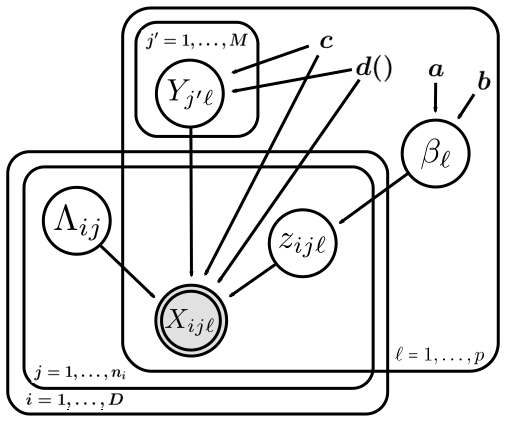
\includegraphics[width=0.35\textwidth]{figures/recordLinkage_graphicalModel}
\caption{Graphical representation of model (\ref{model:string_spec}).}
\label{fig:graphicalProcess}
\end{center}
\end{figure}

\end{document}

